%!TeX jobName=challenges/stego/beatles
%\nofiles
% Created by Bonita Graham
% Last update: February 2019 By Kestutis Bendinskas
%https://es.overleaf.com/gallery/tagged/academic-journal
% Authors:
% Please do not make changes to the preamble until after the solid line of %s.

\documentclass[letterpaper,10pt]{article}
\usepackage[spanish,es-noshorthands]{babel}
\usepackage[latin1,utf8]{inputenc} % Codificación UTF-8

\usepackage[explicit]{titlesec}
\setlength{\parindent}{0pt}
\setlength{\parskip}{1em}
\usepackage{hyphenat}
\usepackage{ragged2e}
%Para colocar puntos en los itemes especiales
\usepackage{pifont}
\RaggedRight

% These commands change the font. If you do not have Garamond on your computer, you will need to install it.
%\usepackage{garamondx}
\usepackage[T1]{fontenc}
\usepackage{amsmath, amsthm}
\usepackage{graphicx}
\usepackage{caption}

% This adjusts the underline to be in keeping with word processors.
\usepackage{soul}
\setul{.6pt}{.4pt}
%This is for the color for the codign
\usepackage[dvipsnames]{xcolor}
%http://latexcolor.com/
\definecolor{almond}{rgb}{0.94, 0.87, 0.8}
\definecolor{airforceblue}{rgb}{0.36, 0.54, 0.66}
\usepackage{listings}

\lstset{
  backgroundcolor=\color{almond}, %color de fondo
  breaklines=true,
  captionpos=b,     % Establece la posición de la leyenda del cuadro de código
  basicstyle=\sffamily,
  %basicstyle=\footnotesize,
  showstringspaces=false,
  commentstyle=\color{red},
  keywordstyle=\color{blue}
}

%https://www.overleaf.com/learn/latex/Hyperlinks
%Styles and colours
\usepackage{hyperref}
\hypersetup{
    colorlinks=true,
    linkcolor=blue,
    filecolor=magenta,
    urlcolor=ForestGreen,
}
\urlstyle{same}

\usepackage{tcolorbox}


% The following sets margins to 1 in. on top and bottom and .75 in on left and right, and remove page numbers.
\usepackage{geometry}
\geometry{vmargin={1in,1in}, hmargin={.75in, .75in}}
\usepackage{fancyhdr}
\pagestyle{fancy}
\pagenumbering{gobble}
\renewcommand{\headrulewidth}{0.0pt}
\renewcommand{\footrulewidth}{0.0pt}

% These Commands create the label style for tables, figures and equations.
\usepackage[labelfont={footnotesize,bf} , textfont=footnotesize]{caption}
\captionsetup{labelformat=simple, labelsep=period}
\newcommand\num{\addtocounter{equation}{1}\tag{\theequation}}
\renewcommand{\theequation}{\arabic{equation}}
\makeatletter
\renewcommand\tagform@[1]{\maketag@@@ {\ignorespaces {\footnotesize{\textbf{Equation}}} #1.\unskip \@@italiccorr }}
\makeatother
\setlength{\intextsep}{10pt}
\setlength{\abovecaptionskip}{2pt}
\setlength{\belowcaptionskip}{-10pt}

\renewcommand{\textfraction}{0.10}
\renewcommand{\topfraction}{0.85}
\renewcommand{\bottomfraction}{0.85}
\renewcommand{\floatpagefraction}{0.90}

% These commands set the paragraph and line spacing
\titleformat{\section}
  {\normalfont}{\thesection}{1em}{\MakeUppercase{\textbf{#1}}}
\titlespacing\section{0pt}{0pt}{-10pt}
\titleformat{\subsection}
  {\normalfont}{\thesubsection}{1em}{\textit{#1}}
\titlespacing\subsection{0pt}{0pt}{-8pt}
\renewcommand{\baselinestretch}{1.15}

% This designs the title display style for the maketitle command
\makeatletter
\newcommand\sixteen{\@setfontsize\sixteen{16pt}{6}}
\renewcommand{\maketitle}{\bgroup\setlength{\parindent}{0pt}
\begin{flushleft}
\vspace{-.375in}
\sixteen\bfseries \@title
\medskip
\end{flushleft}
\textsc{\@author}\\
\textit{\today}
\egroup}
\makeatother

% This styles the bibliography and citations.
%\usepackage[biblabel]{cite}
\usepackage[sort&compress]{natbib}
\setlength\bibindent{2em}
\makeatletter
\renewcommand\@biblabel[1]{\textbf{#1.}\hfill}
\makeatother
\renewcommand{\citenumfont}[1]{\textbf{#1}}
\bibpunct{}{}{,~}{s}{,}{,}
\setlength{\bibsep}{0pt plus 0.3ex}

\renewcommand*{\lstlistingname}{Código}  %CAMBIA EL TITULO DE LISTING EN EL CODIGO


%%%%%%%%%%%%%%%%%%%%%%%%%%%%%%%%%%%%%%%%%%%%%%%%%

% Authors: Add additional packages and new commands here.
% Limit your use of new commands and special formatting.

% Place your title below. Use Title Capitalization.
\title{Write-up: HackTheBox - Crypto - Classic, yet complicated!}

% Add author information below. Communicating author is indicated by an asterisk, the affiliation is shown by superscripted lower case letter if several affiliations need to be noted.
\author{Sebastián Sepúlveda @piblack}


\pagestyle{empty}
\begin{document}

% Makes the title and author information appear.
\vspace*{.01 in}
\maketitle
\vspace{.12 in}

% Start the main part of the manuscript here.
% Comment out section headings if inappropriate to your discipline.
% If you add additional section or subsection headings, use an asterisk * to avoid numbering.

\textbf{Información:} Categoria Crypto, 10 points.

\textbf{Descripción:} Find the plaintext, the key is your flag! Flag format : HTB{key in lowercase}

\section*{WriteUp}

Cuando archivo .zip nos entrega el siguiente texto cifrado:

\begin{tcolorbox}
alp gwcsepul gtavaf, nlv prgpbpsu mb h jcpbyvdlq, ipltga rv glniypfa we ekl 16xs nsjhlcb. px td o lccjdstslpahzn fptspf xstlxzi te iosj ezv sc xcns ttsoic lzlvrmhaw ez sjqijsa xsp rwhr. tq vxspf sciov, alp wsphvcv pr ess rwxpqlvp nwlvvc dyi dswbhvo ef htqtafvyw hqzfbpg, ezutewwm zcep xzmyr o scio ry tscoos rd woi pyqnmgelvr vpm . qbctnl xsp akbflowllmspwt nlwlpcg, lccjdstslpahzn fptspfo oip qvx dfgysgelipp ec bfvbxlrnj ojocjvpw, ld akfv ekhr zys hskehy my eva dclluxpih yoe mh yiacsoseehk fj l gebxwh sieesn we ekl iynfudktru. xsp yam zd woi qwoc.
\end{tcolorbox}

Para saber qué tipo de cifrado es, ocupamos \href{http://mtk911.cf/cipher/}{MTH911}.

\begin{figure}[h]
  \centering
  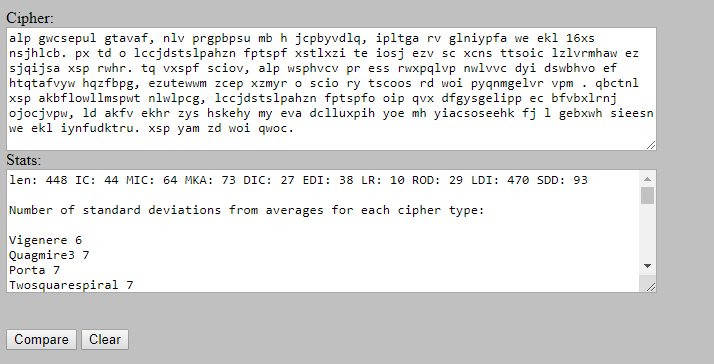
\includegraphics[scale=0.9]{images/classic/classic1}
  \captionof{figure}{Return Cipher Statics}
  \label{fig:classic1}
\end{figure}

Nos dice que es un cifrado \texttt{Vigenere}. Buscando en google, es posible encontrar el siguiente \href{https://www.dcode.fr/vigenere-cipher}{Vigener Cipher}, el que nos facilita las cosas al tener una opción de descriptación automática. Al insertar el texto, colocamos \texttt{THE} en ``KNOWNING A PLAINTEXT WORD'', pues inferimos en el primer intento que el texto está en inglés. la flag en el primer resultado que nos entrega la decodificación. Ver Figura \ref{fig:clasic}:
\newpage
\begin{figure}[h]
  \centering
  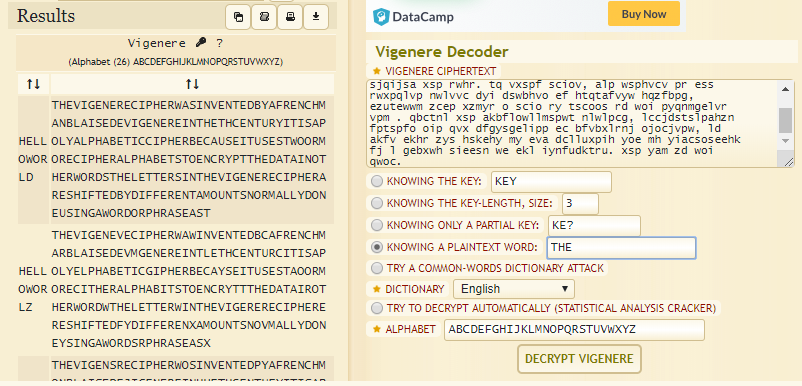
\includegraphics[scale=0.8]{images/classic/classic}
  \captionof{figure}{Flag encontrada}
  \label{fig:clasic}
\end{figure}

\textbf{Flag: }HTB\{helloworld\}

\end{document}


%%TIPOS DE CAJAS

\noindent\fbox{%
    \parbox{\textwidth}{%
alp gwcsepul gtavaf, nlv prgpbpsu mb h jcpbyvdlq, ipltga rv glniypfa we ekl 16xs nsjhlcb. px td o lccjdstslpahzn fptspf xstlxzi te iosj ezv sc xcns ttsoic lzlvrmhaw ez sjqijsa xsp rwhr. tq vxspf sciov, alp wsphvcv pr ess rwxpqlvp nwlvvc dyi dswbhvo ef htqtafvyw hqzfbpg, ezutewwm zcep xzmyr o scio ry tscoos rd woi pyqnmgelvr vpm . qbctnl xsp akbflowllmspwt nlwlpcg, lccjdstslpahzn fptspfo oip qvx dfgysgelipp ec bfvbxlrnj ojocjvpw, ld akfv ekhr zys hskehy my eva dclluxpih yoe mh yiacsoseehk fj l gebxwh sieesn we ekl iynfudktru. xsp yam zd woi qwoc.
}%
}